\documentclass[11pt]{exam}

\usepackage{amssymb, amsmath, amsthm, mathrsfs, multicol, graphicx}
\usepackage{tikz, pgfplots}


\def\d{\displaystyle}
\def\?{\reflectbox{?}}
\def\b#1{\mathbf{#1}}
\def\f#1{\mathfrak #1}
\def\c#1{\mathcal #1}
\def\s#1{\mathscr #1}
\def\r#1{\mathrm{#1}}
\def\N{\mathbb N}
\def\Z{\mathbb Z}
\def\Q{\mathbb Q}
\def\R{\mathbb R}
\def\C{\mathbb C}
\def\F{\mathbb F}
\def\A{\mathbb A}
\def\X{\mathbb X}
\def\E{\mathbb E}
\def\O{\mathbb O}
\def\pow{\mathscr P}
\def\inv{^{-1}}
\def\nrml{\triangleleft}
\def\st{:}
\def\~{\widetilde}
\def\rem{\mathcal R}
\def\iff{\leftrightarrow}
\def\Iff{\Leftrightarrow}
\def\and{\wedge}
\def\And{\bigwedge}
\def\AAnd{\d\bigwedge\mkern-18 mu\bigwedge}
\def\Vee{\bigvee}
\def\VVee{\d\Vee\mkern-18 mu\Vee}
\def\imp{\rightarrow}
\def\Imp{\Rightarrow}
\def\Fi{\Leftarrow}



\def\circleA{(-.5,0) circle (1)}
\def\circleAlabel{(-1.5,.6) node[above]{$A$}}
\def\circleB{(.5,0) circle (1)}
\def\circleBlabel{(1.5,.6) node[above]{$B$}}
\def\circleC{(0,-1) circle (1)}
\def\circleClabel{(.5,-2) node[right]{$C$}}
\def\twosetbox{(-2,-1.5) rectangle (2,1.5)}
\def\threesetbox{(-2,-2.5) rectangle (2,1.5)}


\def\bar{\overline}

%\pointname{pts}
\pointsinmargin
\marginpointname{pts}
\marginbonuspointname{ bns pts}

\addpoints
\pagestyle{headandfoot}
%\printanswers


\header{MATH 131}{\bf\large Learning Target 4 Quiz}{Fall 2025}
\runningfooter{}{}{Version \version}
\extrafootheight{-.45 in}


\begin{document}
\def\version{A}
%space for name
\noindent {\large\bf Name:} \underline{\hspace{2.5 in}}
\vskip 1em

\pgfplotsset{every tick label/.append style={font=\tiny, fill=white, fill}}

\begin{questions}
  \question For each function graphed below, carefully sketch a graph of the functions derivative in the space provided below the original graph. 
  \begin{multicols}{2}
    % First function
        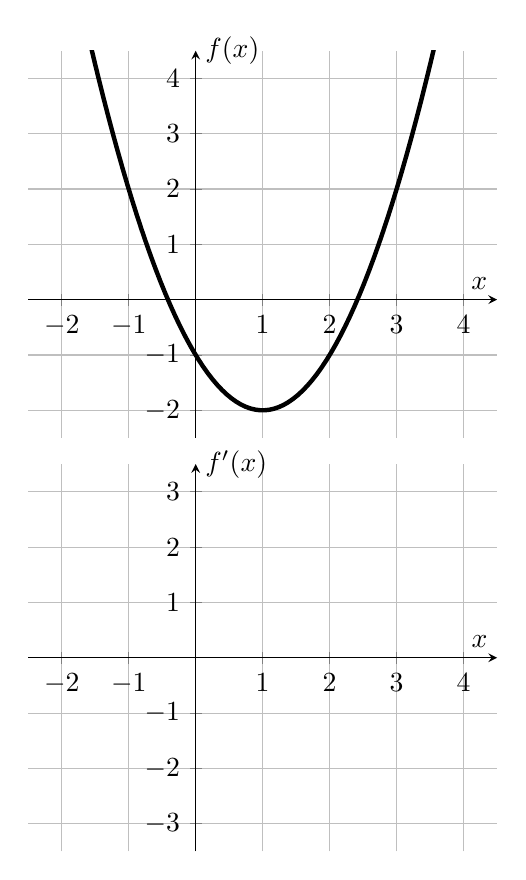
\begin{tikzpicture}[
      declare function={
        func(\x)= ( \x - 1)^2 - 2;
      }
    ]
      \begin{axis}[height=6.5cm,
        axis lines=center, ymin=-2.5, ymax=4.5, xmin=-2.5, xmax=4.5, xlabel=$x$, ylabel=$f(x)$, ylabel style={right}, ytick={-2,-1,...,4}, xtick={-4,-3,...,4}, grid=both
      ]
        \addplot [domain=-3:4,samples=100, ultra thick]{func(x)};
      \end{axis}
        \begin{axis}[height=6.5cm, yshift=-5.25cm,
        axis lines=center, ymin=-3.5, ymax=3.5, xmin=-2.5, xmax=4.5, xlabel=$x$, ylabel=$f'(x)$, ylabel style={right}, ytick={-3,-2,-1,...,4}, xtick={-4,-3,...,4}, grid=both
      ]
      \end{axis}  

    \end{tikzpicture}
    
\vskip 1em
        % Second function
        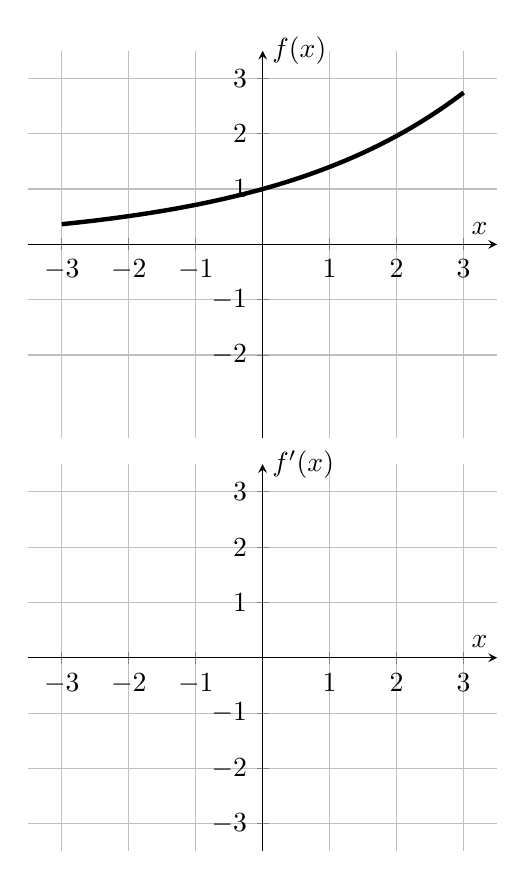
\begin{tikzpicture}[
      declare function={
        func(\x)= 1.4^\x;
      }
    ]
      \begin{axis}[height=6.5cm,
        axis lines=center, ymin=-3.5, ymax=3.5, xmin=-3.5, xmax=3.5, xlabel=$x$, ylabel=$f(x)$, ylabel style={right}, ytick={-2,-1,...,4}, xtick={-4,-3,...,4}, grid=both
      ]
        \addplot [domain=-3:3,samples=100, ultra thick]{func(x)};
      \end{axis}
        \begin{axis}[height=6.5cm, yshift=-5.25cm,
        axis lines=center, ymin=-3.5, ymax=3.5, xmin=-3.5, xmax=3.5, xlabel=$x$, ylabel=$f'(x)$, ylabel style={right}, ytick={-3,-2,-1,...,4}, xtick={-4,-3,...,4}, grid=both
      ]
      \end{axis}  

    \end{tikzpicture}
    

    \columnbreak

        % Third function
        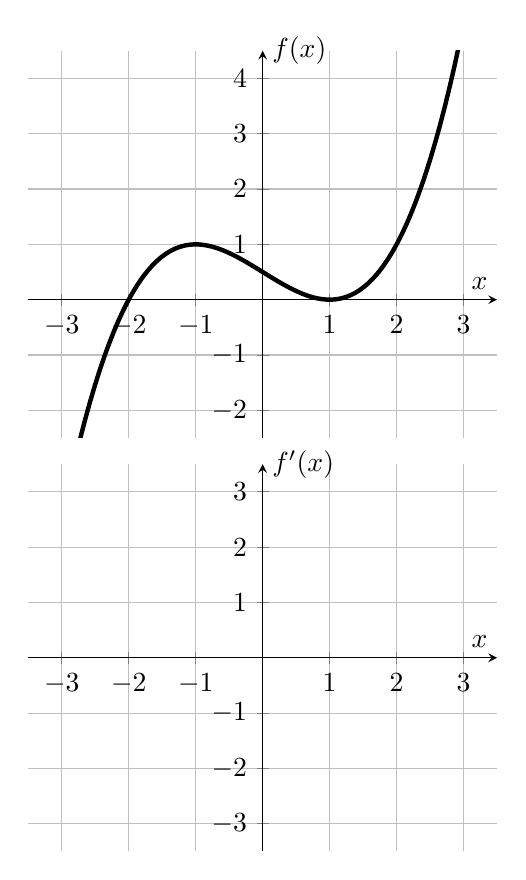
\begin{tikzpicture}[
      declare function={
        func(\x)= .25*( \x^3 - 3*\x + 2 );
      }
    ]
      \begin{axis}[height=6.5cm,
        axis lines=center, ymin=-2.5, ymax=4.5, xmin=-3.5, xmax=3.5, xlabel=$x$, ylabel=$f(x)$, ylabel style={right}, ytick={-2,-1,...,4}, xtick={-4,-3,...,4}, grid=both
      ]
        \addplot [domain=-3.5:3.5,samples=100, ultra thick]{func(x)};
      \end{axis}
      \begin{axis}[height=6.5cm, yshift=-5.25cm,
        axis lines=center, ymin=-3.5, ymax=3.5, xmin=-3.5, xmax=3.5, xlabel=$x$, ylabel=$f'(x)$, ylabel style={right}, ytick={-3,-2,-1,...,4}, xtick={-4,-3,...,4}, grid=both
      ]
      \end{axis}  

    \end{tikzpicture}
    
\vskip .5em
        
        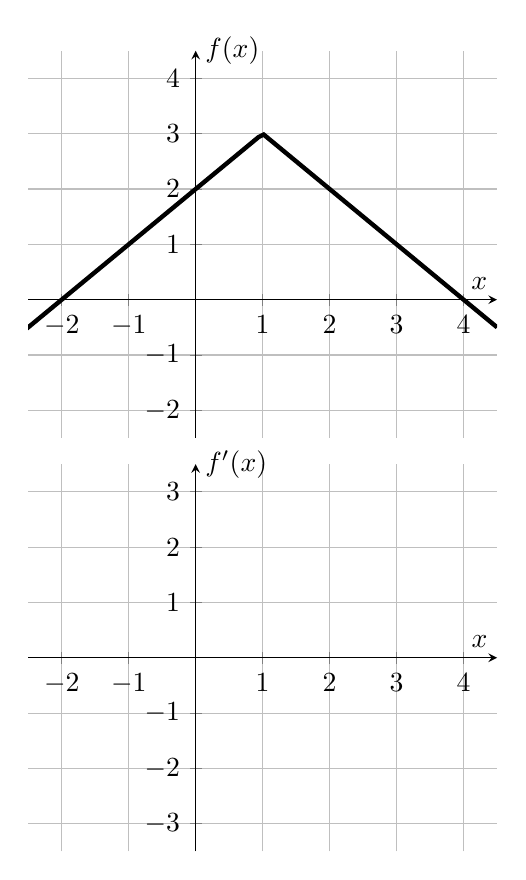
\begin{tikzpicture}[
      declare function={
        func(\x)= -1*abs(x-1)+3;
      }
    ]
      \begin{axis}[height=6.5cm,
        axis lines=center, ymin=-2.5, ymax=4.5, xmin=-2.5, xmax=4.5, xlabel=$x$, ylabel=$f(x)$, ylabel style={right}, ytick={-2,-1,...,4}, xtick={-4,-3,...,4}, grid=both
      ]
        \addplot [domain=-3:4.5,samples=100, ultra thick]{func(x)};
      \end{axis}
        \begin{axis}[height=6.5cm, yshift=-5.25cm,
        axis lines=center, ymin=-3.5, ymax=3.5, xmin=-2.5, xmax=4.5, xlabel=$x$, ylabel=$f'(x)$, ylabel style={right}, ytick={-3,-2,-1,...,4}, xtick={-4,-3,...,4}, grid=both
      ]
      \end{axis}  

    \end{tikzpicture}
    
  \end{multicols}
\end{questions}



\newpage

\def\version{B}
%space for name
\noindent {\large\bf Name:} \underline{\hspace{2.5 in}}
\vskip 1em

\begin{questions}
  \question For each function graphed below, carefully sketch a graph of the functions derivative in the space provided below the original graph. 
  \begin{multicols}{2}
    % First function
            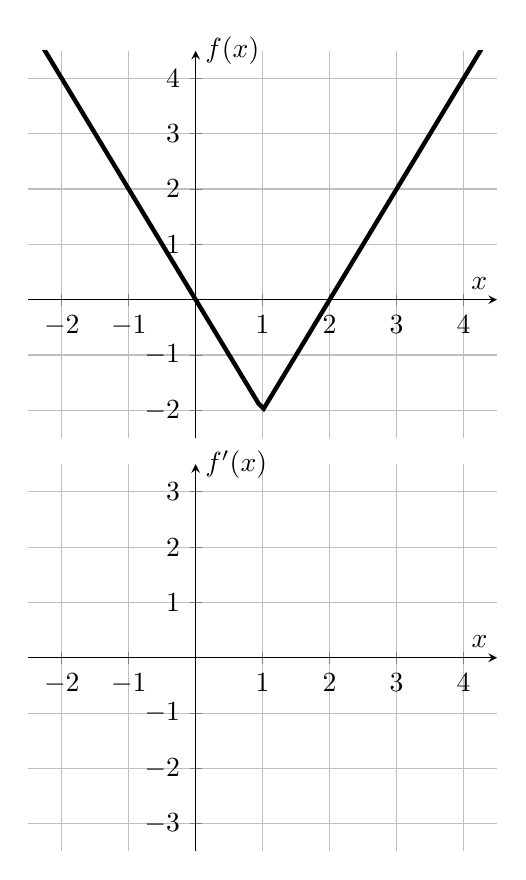
\begin{tikzpicture}[
      declare function={
        func(\x)= 2*abs(x-1)-2;
      }
    ]
      \begin{axis}[height=6.5cm,
        axis lines=center, ymin=-2.5, ymax=4.5, xmin=-2.5, xmax=4.5, xlabel=$x$, ylabel=$f(x)$, ylabel style={right}, ytick={-2,-1,...,4}, xtick={-4,-3,...,4}, grid=both
      ]
        \addplot [domain=-3:4.5,samples=100, ultra thick]{func(x)};
      \end{axis}
        \begin{axis}[height=6.5cm, yshift=-5.25cm,
        axis lines=center, ymin=-3.5, ymax=3.5, xmin=-2.5, xmax=4.5, xlabel=$x$, ylabel=$f'(x)$, ylabel style={right}, ytick={-3,-2,-1,...,4}, xtick={-4,-3,...,4}, grid=both
      ]
      \end{axis}  

    \end{tikzpicture}
    \vskip 1em
    % Second function
    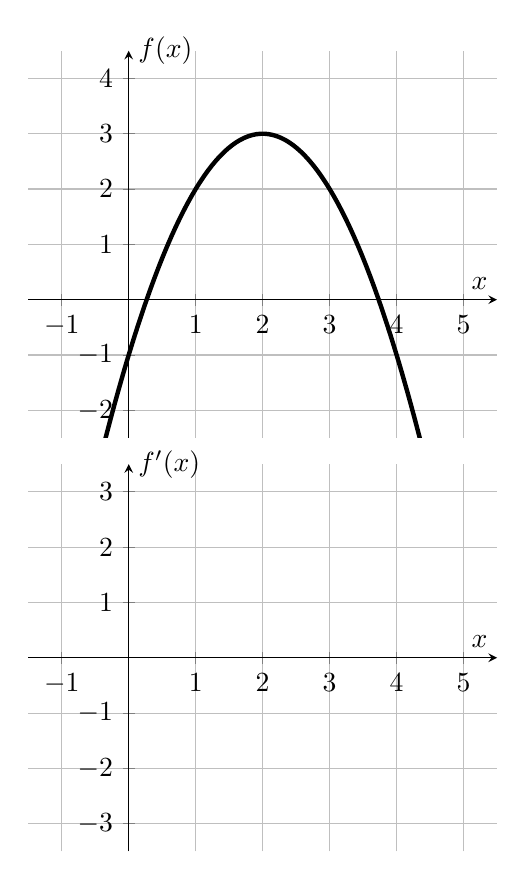
\begin{tikzpicture}[
      declare function={
        func(\x)= -1*(\x - 2)^2 + 3;
      }
    ]
      \begin{axis}[height=6.5cm,
        axis lines=center, ymin=-2.5, ymax=4.5, xmin=-1.5, xmax=5.5, xlabel=$x$, ylabel=$f(x)$, ylabel style={right}, ytick={-2,-1,...,4}, xtick={-4,-3,...,5}, grid=both
      ]
        \addplot [domain=-1:5,samples=100, ultra thick]{func(x)};
      \end{axis}
        \begin{axis}[height=6.5cm, yshift=-5.25cm,
        axis lines=center, ymin=-3.5, ymax=3.5, xmin=-1.5, xmax=5.5, xlabel=$x$, ylabel=$f'(x)$, ylabel style={right}, ytick={-3,-2,-1,...,4}, xtick={-4,-3,...,5}, grid=both
      ]
      \end{axis}  

    \end{tikzpicture}
    
    
    
    \columnbreak
    
    % Third function
    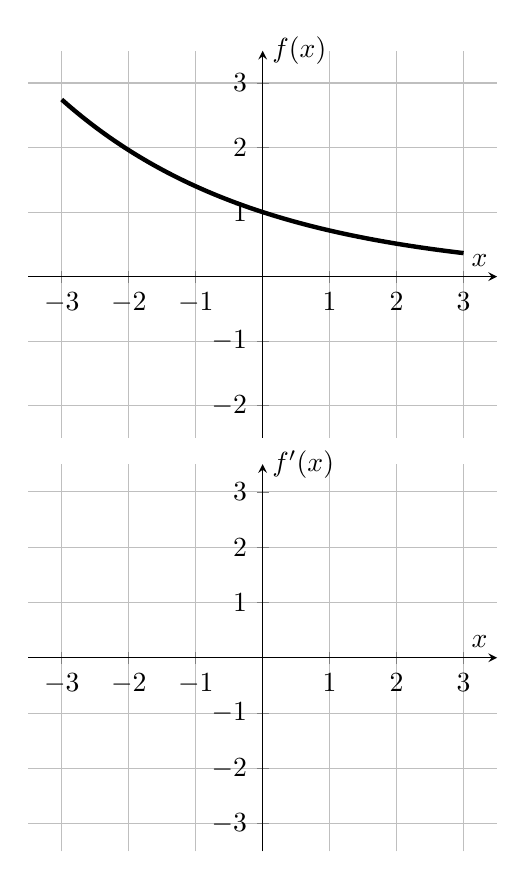
\begin{tikzpicture}[
      declare function={
        func(\x)= 1.4^(-\x);
      }
    ]
      \begin{axis}[height=6.5cm,
        axis lines=center, ymin=-2.5, ymax=3.5, xmin=-3.5, xmax=3.5, xlabel=$x$, ylabel=$f(x)$, ylabel style={right}, ytick={-2,-1,...,4}, xtick={-4,-3,...,4}, grid=both
      ]
        \addplot [domain=-3:3,samples=100, ultra thick]{func(x)};
      \end{axis}
        \begin{axis}[height=6.5cm, yshift=-5.25cm,
        axis lines=center, ymin=-3.5, ymax=3.5, xmin=-3.5, xmax=3.5, xlabel=$x$, ylabel=$f'(x)$, ylabel style={right}, ytick={-3,-2,-1,...,4}, xtick={-4,-3,...,4}, grid=both
      ]
      \end{axis}  

    \end{tikzpicture}
    
    \vskip .5em

    % Fourth    
    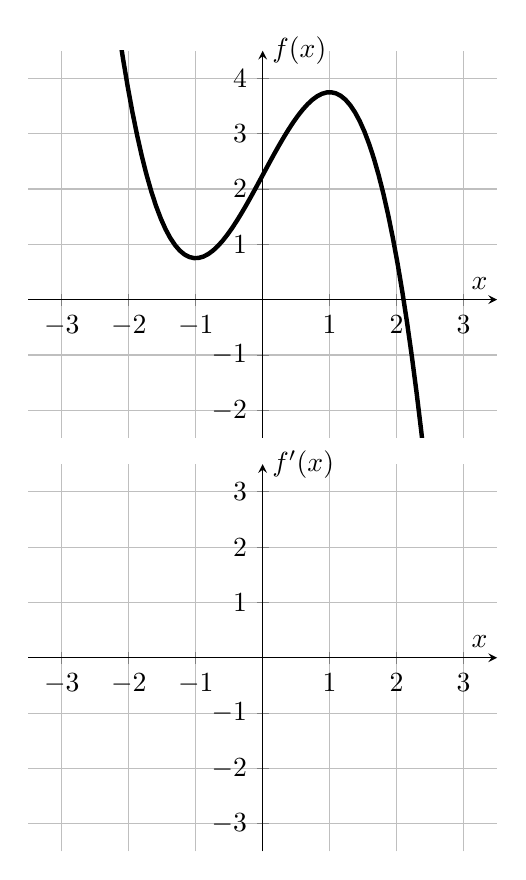
\begin{tikzpicture}[
  declare function={
    func(\x)= .75*( -\x^3 + 3*\x + 3 );
  }
]
  \begin{axis}[height=6.5cm,
    axis lines=center, ymin=-2.5, ymax=4.5, xmin=-3.5, xmax=3.5, xlabel=$x$, ylabel=$f(x)$, ylabel style={right}, ytick={-2,-1,...,4}, xtick={-4,-3,...,4}, grid=both
  ]
    \addplot [domain=-3.5:3.5,samples=100, ultra thick]{func(x)};
  \end{axis}
  \begin{axis}[height=6.5cm, yshift=-5.25cm,
    axis lines=center, ymin=-3.5, ymax=3.5, xmin=-3.5, xmax=3.5, xlabel=$x$, ylabel=$f'(x)$, ylabel style={right}, ytick={-3,-2,-1,...,4}, xtick={-4,-3,...,4}, grid=both
  ]
  \end{axis}  

\end{tikzpicture}
    
    
  \end{multicols}
\end{questions}


\newpage

\def\version{C}
%space for name
\noindent {\large\bf Name:} \underline{\hspace{2.5 in}}
\vskip 1em

\begin{questions}
  \question For each function graphed below, carefully sketch a graph of the functions derivative in the space provided below the original graph. 
  \begin{multicols}{2}
    % First function 
     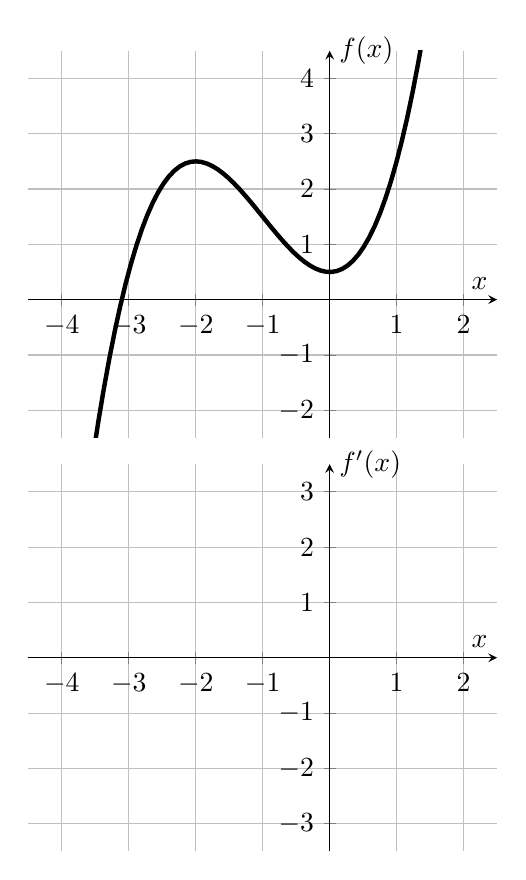
\begin{tikzpicture}[
      declare function={
        func(\x)= .5*( (\x+1)^3 - 3*(\x+1) + 3 );
      }
    ]
      \begin{axis}[height=6.5cm,
        axis lines=center, ymin=-2.5, ymax=4.5, xmin=-4.5, xmax=2.5, xlabel=$x$, ylabel=$f(x)$, ylabel style={right}, ytick={-2,-1,...,4}, xtick={-4,-3,...,4}, grid=both
      ]
        \addplot [domain=-4.5:3.5,samples=100, ultra thick]{func(x)};
      \end{axis}
      \begin{axis}[height=6.5cm, yshift=-5.25cm,
        axis lines=center, ymin=-3.5, ymax=3.5, xmin=-4.5, xmax=2.5, xlabel=$x$, ylabel=$f'(x)$, ylabel style={right}, ytick={-3,-2,-1,...,4}, xtick={-4,-3,...,4}, grid=both
      ]
      \end{axis}  

    \end{tikzpicture}

    
\vskip 1em
        % Second function

        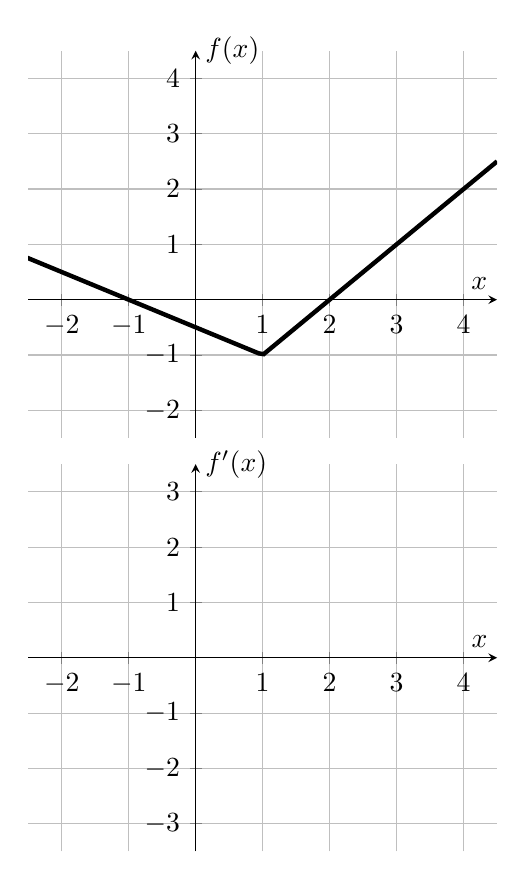
\begin{tikzpicture}[
      declare function={
        func(\x)= (-0.5*\x -0.5) * (x < 1) + (\x-2) * (x > 1);
      }
    ]
      \begin{axis}[height=6.5cm,
        axis lines=center, ymin=-2.5, ymax=4.5, xmin=-2.5, xmax=4.5, xlabel=$x$, ylabel=$f(x)$, ylabel style={right}, ytick={-2,-1,...,4}, xtick={-4,-3,...,4}, grid=both
      ]
        \addplot [domain=-3:4.5,samples=100, ultra thick]{func(x)};
      \end{axis}
        \begin{axis}[height=6.5cm, yshift=-5.25cm,
        axis lines=center, ymin=-3.5, ymax=3.5, xmin=-2.5, xmax=4.5, xlabel=$x$, ylabel=$f'(x)$, ylabel style={right}, ytick={-3,-2,-1,...,4}, xtick={-4,-3,...,4}, grid=both
      ]
      \end{axis}  

    \end{tikzpicture}


    

    \columnbreak

        % Third function
        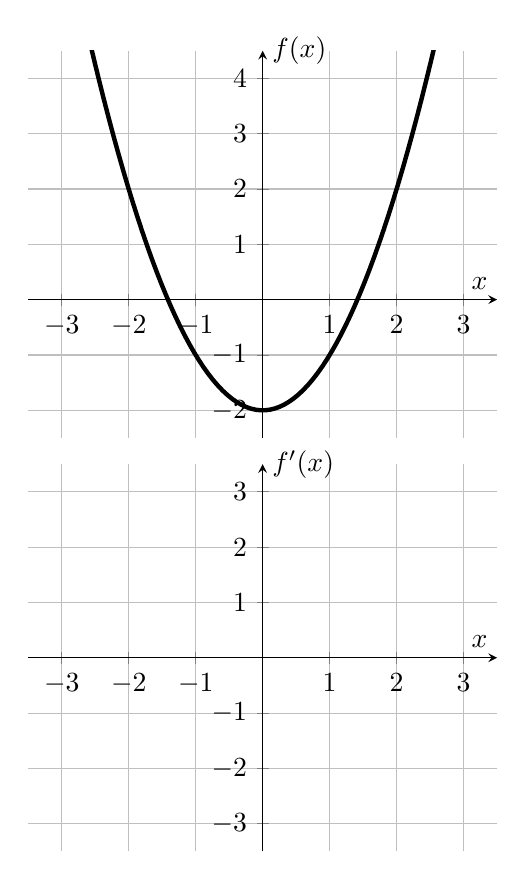
\begin{tikzpicture}[
      declare function={
        func(\x)= (\x)^2 - 2;
      }
    ]
      \begin{axis}[height=6.5cm,
        axis lines=center, ymin=-2.5, ymax=4.5, xmin=-3.5, xmax=3.5, xlabel=$x$, ylabel=$f(x)$, ylabel style={right}, ytick={-2,-1,...,4}, xtick={-4,-3,...,4}, grid=both
      ]
        \addplot [domain=-3:4,samples=100, ultra thick]{func(x)};
      \end{axis}
        \begin{axis}[height=6.5cm, yshift=-5.25cm,
        axis lines=center, ymin=-3.5, ymax=3.5, xmin=-3.5, xmax=3.5, xlabel=$x$, ylabel=$f'(x)$, ylabel style={right}, ytick={-3,-2,-1,...,4}, xtick={-4,-3,...,4}, grid=both
      ]
      \end{axis}  

    \end{tikzpicture}
    
\vskip .5em

        % Fourth
        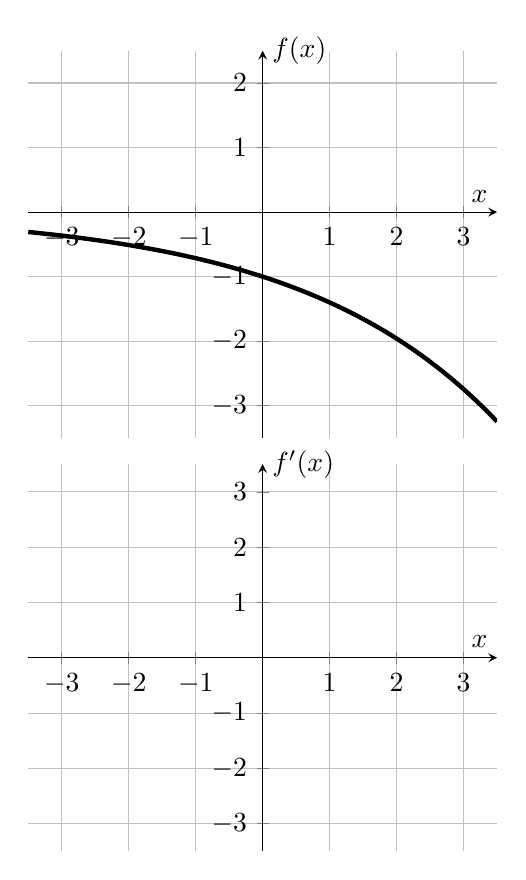
\begin{tikzpicture}[
      declare function={
        func(\x)= -1.4^\x;
      }
    ]
      \begin{axis}[height=6.5cm,
        axis lines=center, ymin=-3.5, ymax=2.5, xmin=-3.5, xmax=3.5, xlabel=$x$, ylabel=$f(x)$, ylabel style={right}, ytick={-3,-2,-1,...,4}, xtick={-4,-3,...,4}, grid=both
      ]
        \addplot [domain=-3.5:3.5,samples=100, ultra thick]{func(x)};
      \end{axis}
        \begin{axis}[height=6.5cm, yshift=-5.25cm,
        axis lines=center, ymin=-3.5, ymax=3.5, xmin=-3.5, xmax=3.5, xlabel=$x$, ylabel=$f'(x)$, ylabel style={right}, ytick={-3,-2,-1,...,4}, xtick={-4,-3,...,4}, grid=both
      ]
      \end{axis}  

    \end{tikzpicture}
    
  \end{multicols}
\end{questions}



\newpage

\def\version{D}
%space for name
\noindent {\large\bf Name:} \underline{\hspace{2.5 in}}
\vskip 1em

\begin{questions}
  \question For each function graphed below, carefully sketch a graph of the functions derivative in the space provided below the original graph. 
  \begin{multicols}{2}
    % First function

        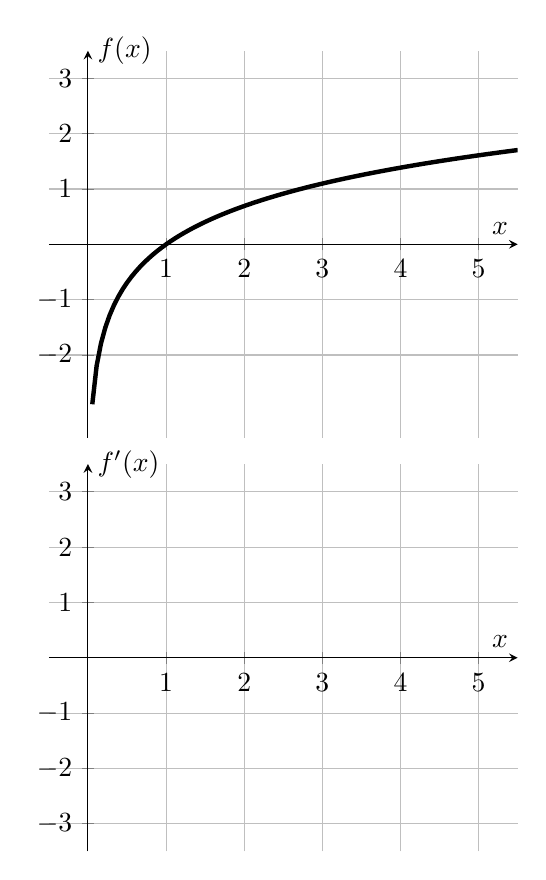
\begin{tikzpicture}[
      declare function={
        func(\x)= ln(\x);
      }
    ]
      \begin{axis}[height=6.5cm,
        axis lines=center, ymin=-3.5, ymax=3.5, xmin=-0.5, xmax=5.5, xlabel=$x$, ylabel=$f(x)$, ylabel style={right}, ytick={-2,-1,...,4}, xtick={-4,-3,...,4,5}, grid=both
      ]
        \addplot [domain=0:5.5,samples=100, ultra thick]{func(x)};
      \end{axis}
        \begin{axis}[height=6.5cm, yshift=-5.25cm,
        axis lines=center, ymin=-3.5, ymax=3.5, xmin=-0.5, xmax=5.5, xlabel=$x$, ylabel=$f'(x)$, ylabel style={right}, ytick={-3,-2,-1,...,4}, xtick={-4,-3,...,4,5}, grid=both
      ]
      \end{axis}  

    \end{tikzpicture}




    
\vskip 1em
        % Second function
        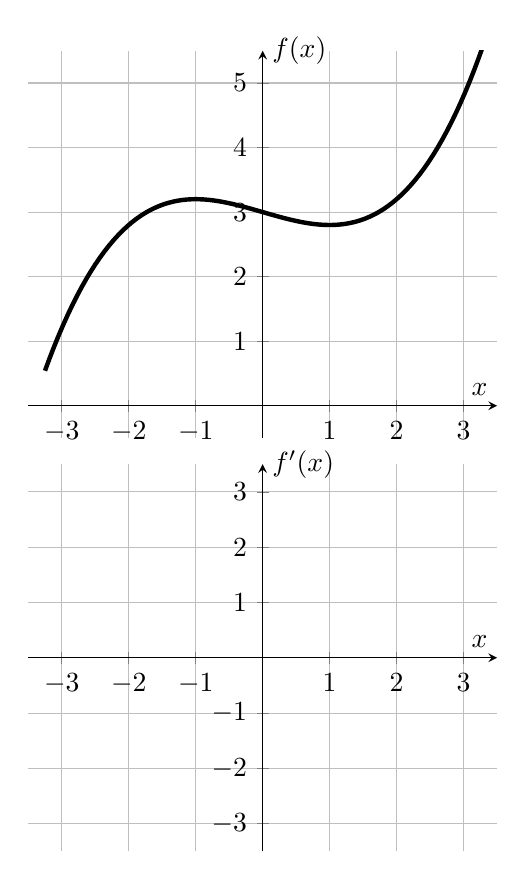
\begin{tikzpicture}[
      declare function={
        func(\x)= .1*( \x^3 - 3*\x ) + 3;
      }
    ]
      \begin{axis}[height=6.5cm,
        axis lines=center, ymin=-0.5, ymax=5.5, xmin=-3.5, xmax=3.5, xlabel=$x$, ylabel=$f(x)$, ylabel style={right}, ytick={-2,-1,...,4,5}, xtick={-4,-3,...,4}, grid=both
      ]
        \addplot [domain=-3.25:3.5,samples=100, ultra thick]{func(x)};
      \end{axis}
      \begin{axis}[height=6.5cm, yshift=-5.25cm,
        axis lines=center, ymin=-3.5, ymax=3.5, xmin=-3.5, xmax=3.5, xlabel=$x$, ylabel=$f'(x)$, ylabel style={right}, ytick={-3,-2,-1,...,4}, xtick={-4,-3,...,4}, grid=both
      ]
      \end{axis}  

    \end{tikzpicture}
    

    \columnbreak

    % Third function

            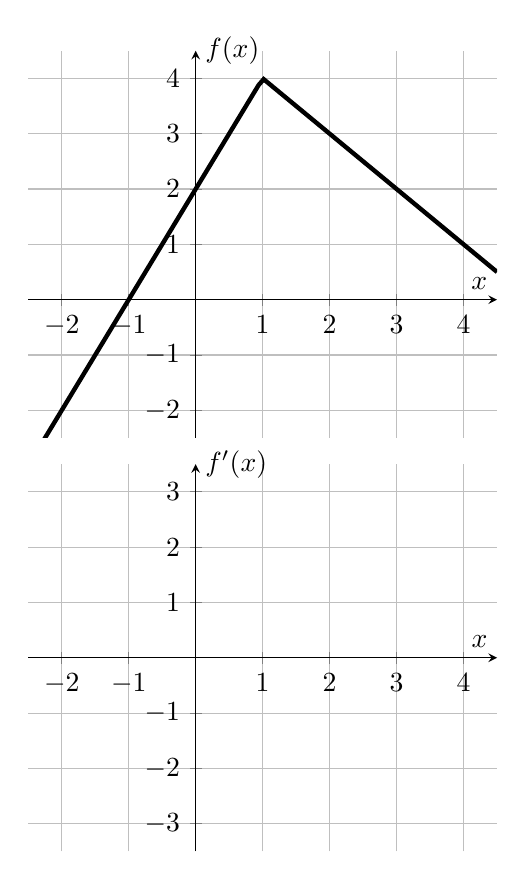
\begin{tikzpicture}[
      declare function={
        func(\x)= (2*x + 2) * (x < 1) + (-1*x +5) * (x >= 1) ;
      }
    ]
      \begin{axis}[height=6.5cm,
        axis lines=center, ymin=-2.5, ymax=4.5, xmin=-2.5, xmax=4.5, xlabel=$x$, ylabel=$f(x)$, ylabel style={right}, ytick={-2,-1,...,4}, xtick={-4,-3,...,4}, grid=both
      ]
        \addplot [domain=-3:4.5,samples=100, ultra thick]{func(x)};
      \end{axis}
        \begin{axis}[height=6.5cm, yshift=-5.25cm,
        axis lines=center, ymin=-3.5, ymax=3.5, xmin=-2.5, xmax=4.5, xlabel=$x$, ylabel=$f'(x)$, ylabel style={right}, ytick={-3,-2,-1,...,4}, xtick={-4,-3,...,4}, grid=both
      ]
      \end{axis}  
    \end{tikzpicture}

    
\vskip .5em
        
        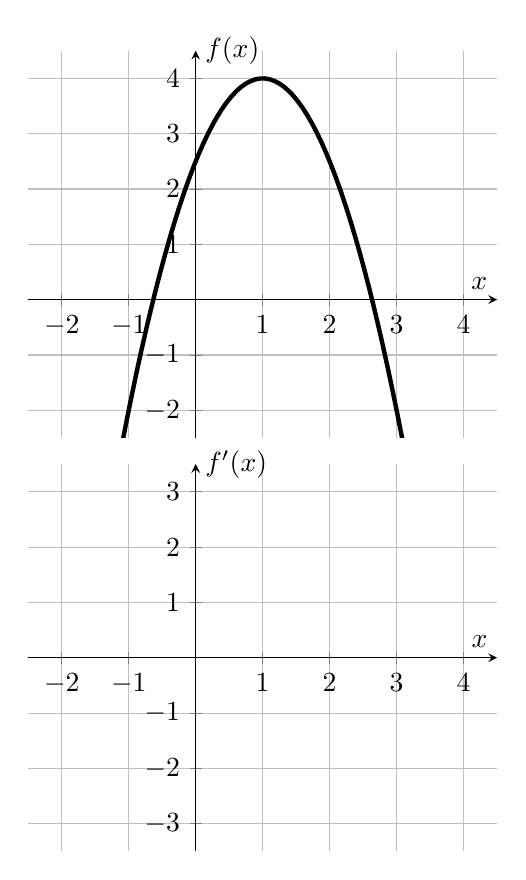
\begin{tikzpicture}[
      declare function={
        func(\x)= -1.5* ( \x - 1)^2 +4 ;
      }
    ]
      \begin{axis}[height=6.5cm,
        axis lines=center, ymin=-2.5, ymax=4.5, xmin=-2.5, xmax=4.5, xlabel=$x$, ylabel=$f(x)$, ylabel style={right}, ytick={-2,-1,...,4}, xtick={-4,-3,...,4}, grid=both
      ]
        \addplot [domain=-3:4,samples=100, ultra thick]{func(x)};
      \end{axis}
        \begin{axis}[height=6.5cm, yshift=-5.25cm,
        axis lines=center, ymin=-3.5, ymax=3.5, xmin=-2.5, xmax=4.5, xlabel=$x$, ylabel=$f'(x)$, ylabel style={right}, ytick={-3,-2,-1,...,4}, xtick={-4,-3,...,4}, grid=both
      ]
      \end{axis}  

    \end{tikzpicture}
    
  \end{multicols}
\end{questions}


\end{document}
